\section{Las aguas continentales}

\subsection{Los ríos}

Los ríos son corrientes naturales y continuas de agua dulce que nacen en zonas montañosas, atraviesan valles y llanuras y desembocan en el mar, en un lago o en otro río. Los ríos que desembocan en otro se denominan afluentes.

\vspace{3mm}
\textbf{Principales elementos de un río} (Figura: \ref{fig:elementos-rio})
\begin{itemize}
    \item \textbf{Nacimiento} es el lugar donde nace o brota.
    \item \textbf{Curso} es el recorrido desde su nacimiento hasta la desembocadura. Se diferencian tres partes:
    \begin{itemize}
        \item \textbf{Curso alto} es el tramo más cercano a su nacimiento. En este tramo, las aguas corren rápidas y arrastran gran cantidad de arena y piedras, produciendo una gran erosión.
        \item \textbf{Curso medio} es el tramo entre el curso alto y el curso bajo. Alterna zonas de fuerte erosión con zonas donde se depositan la arena y las piedras debido a los cambios de la pendiente.
        \item \textbf{Curso bajo} es el tramo próximo a la desembocadura. En esta zona, la pendiente es casi nula y presenta meandros o grandes curvaturas. Debido a la acumulación de los materiales en este tramo se forman deltas y estuarios.
    \end{itemize}
    \item \textbf{Cauce} es el terreno por donde discurren las aguas del río.
\end{itemize}

\begin{figure}[!ht]
    \centering
    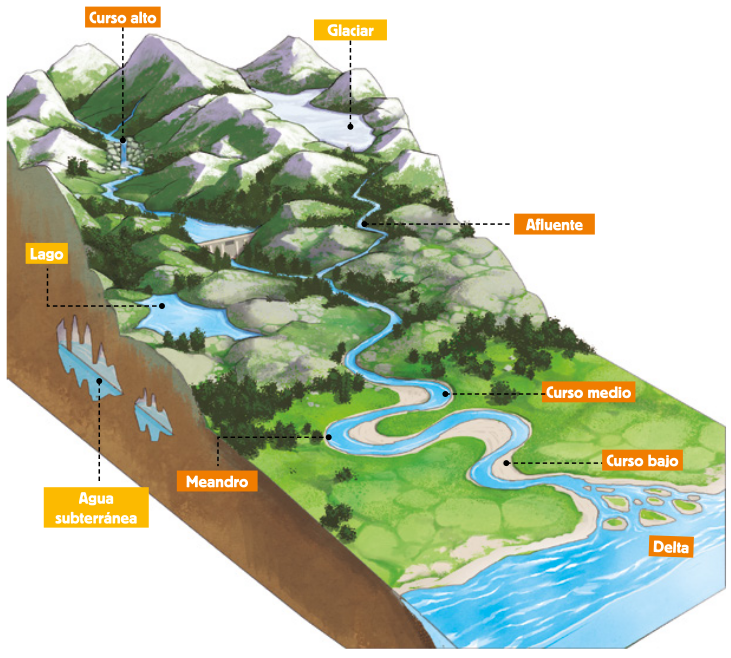
\includegraphics[width=0.7\linewidth]{Tema2/07_Aguas_continentales.png}
    \caption{Elementos de un río}
    \label{fig:elementos-rio}
\end{figure}

\textbf{Principales características de un río}

\begin{itemize}
    \item \textbf{Longitud} es la distancia entre su nacimiento y la desembocadura.
    \item \textbf{Caudal} es la cantidad de agua que lleva un río en un lugar y momento determinado.
    \item \textbf{Régimen} es la variación de caudal a lo largo del año. Es regular cuando no varía a lo largo del año, e irregular, cuando sufre grandes crecidas en épocas de lluvia y está casi seco durante el resto del año.
\end{itemize}
Estas características diferencian a un río de otro, debido principalmente a dos factores: el relieve y el clima.
\begin{itemize}
    \item El \textbf{relieve} influye en la longitud y la velocidad de las aguas del río. Los ríos son más largos cuanto más alejadas están las montañas donde nacen del mar en que desembocan.
    \item El \textbf{clima} repercute en el caudal y el régimen de los ríos. Así, los ríos que atraviesan zonas lluviosas son muy caudalosos y tienen régimen regular. Sin embargo, los ríos que discurren por zonas con climas secos tienen un régimen irregular.
\end{itemize}

\subsection{Otras aguas}

\begin{itemize}
    \item \textbf{Glaciares}

    Son grandes acumulaciones de hielo. Se encuentran en los polos y en la alta montaña.
    \item \textbf{Lagos}
    
    Son acumulaciones de agua en depresiones del relieve. Cuando estas son más pequeñas se llaman lagunas.
    \item \textbf{Acuíferos}

    Son acumulaciones de agua subterránea. Se forman por las filtraciones de agua desde la superficie terrestre.
\end{itemize}